\documentclass{article}

\usepackage{graphicx}
\usepackage{tikz}
\usepackage{tikzsymbols}
\usetikzlibrary{calc,patterns,shapes.geometric}
\pagestyle{empty}
\usepackage[margin=0pt]{geometry}
\geometry{papersize={14in,12in}}

\def\centerarc[#1](#2)(#3:#4:#5){\draw[#1] ($(#2)+({#5*cos(#3)},{#5*sin(#3)})$) arc (#3:#4:#5);}

\begin{document}
	\begin{figure}
		\centering
		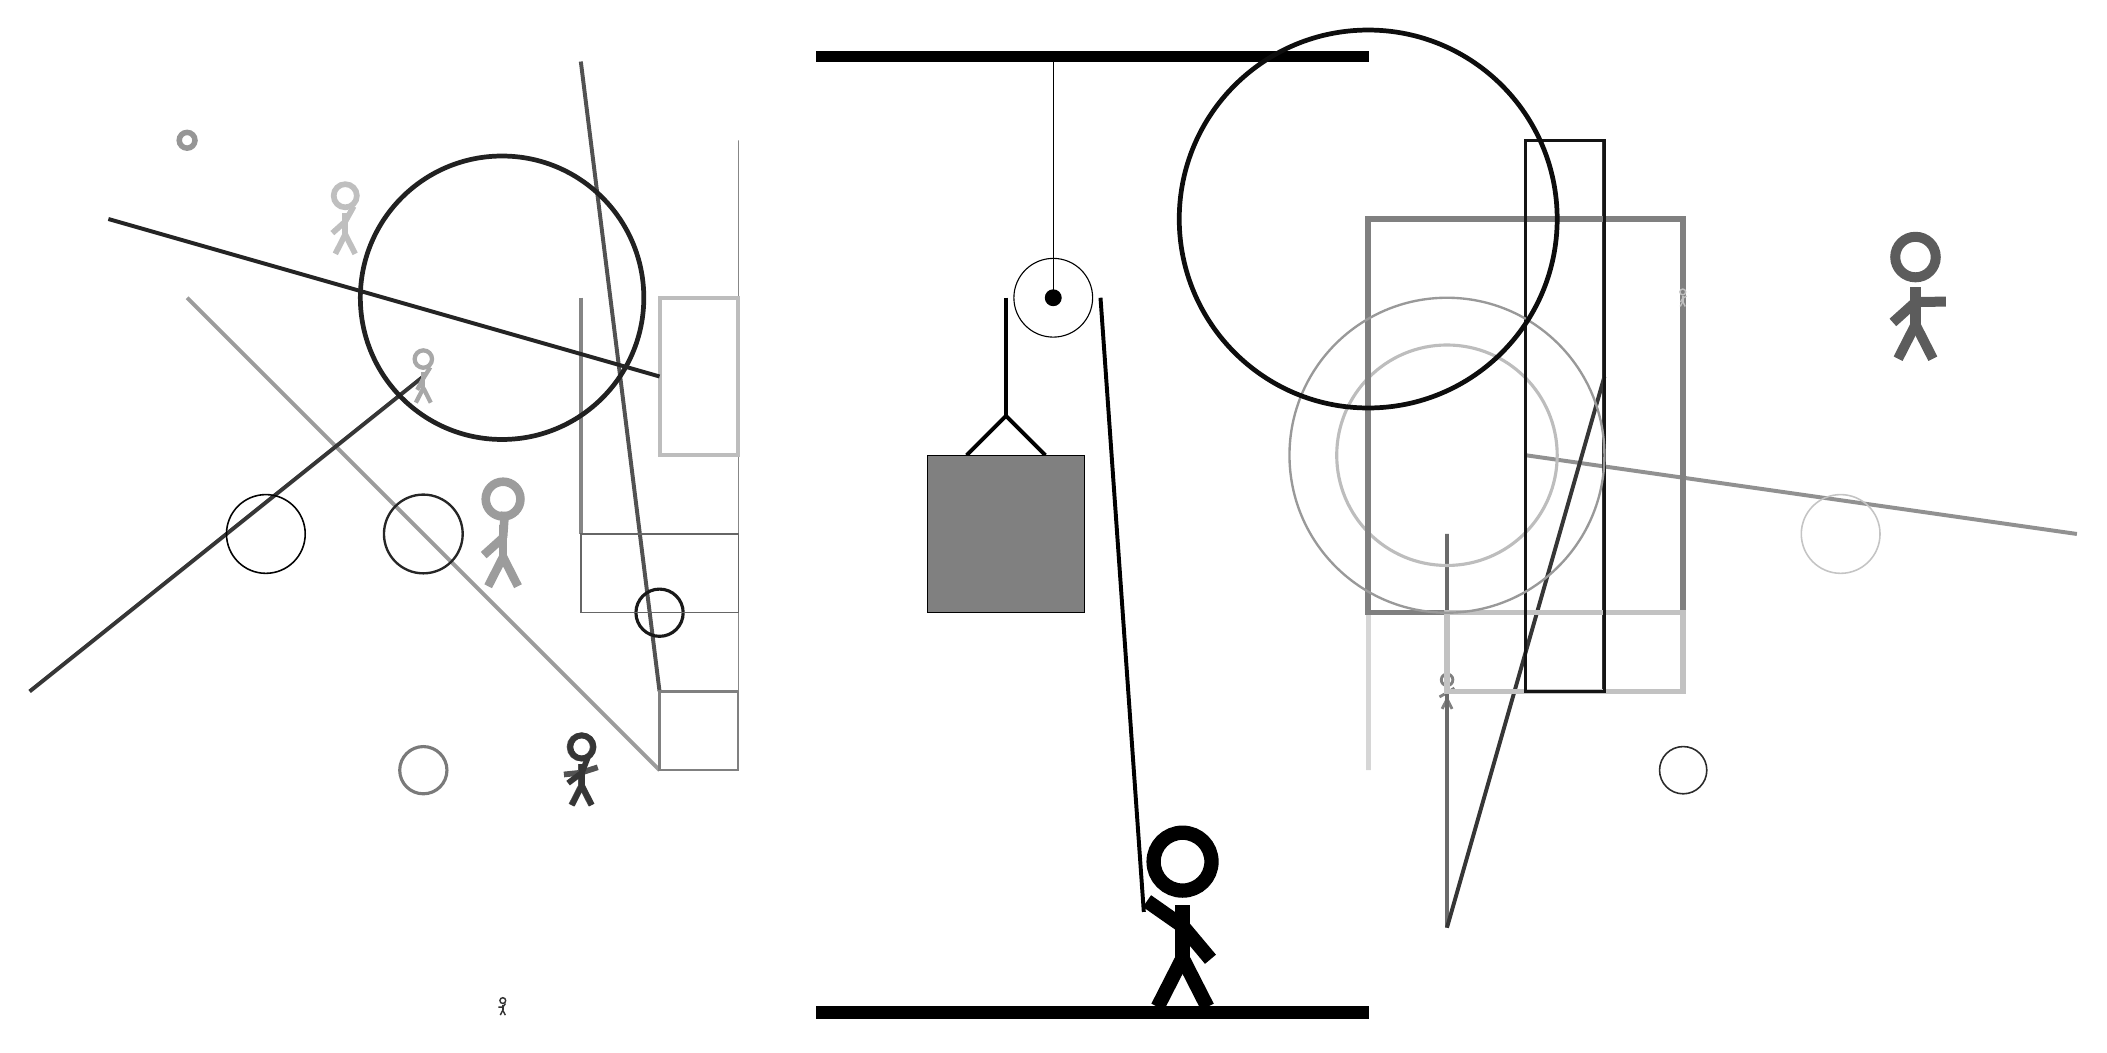
\begin{tikzpicture}
			%%%%% START %%%%%
			
			\draw[fill=black] (-2, 9) rectangle (5, 9.125);
			
			\draw (1, 6) circle (0.5);
			\draw[fill=black] (1, 6) circle (0.1);
			\draw (1, 9) -- (1, 6);
			
			\draw[line width=0.5mm] (-0.1, 4.0) -- (0.4, 4.5) -- (0.9, 4.0);
			\draw[fill=black!50] (-0.6, 4.0) rectangle (1.4, 2.0);
			
			\draw[line width=0.5mm, color=black!43](7, 4) -- (14, 3);
			
			\node[line width=0.4mm, color=black!50] at (6, 1) {\Strichmaxerl[2][29][32]};
			\draw[line width=0.5mm, color=black!39](-4, 0) -- (-10, 6);
			\draw [line width=0.2mm, color=black!23](11, 3) circle (0.5);
			\draw[line width=0.5mm, color=black!68](-5, 9) -- (-4, 1);
			
			\node[line width=0.5mm, color=black!80] at (-6, -3) {\Strichmaxerl[1][1][52]};
			
			\draw [line width=0.4mm, color=black!90](-4, 2) circle (0.3);
			\draw[line width=0.6mm, color=black!16] (5, 0) rectangle (5, 3);
			\draw [line width=0.3mm, color=black!85](-7, 3) circle (0.5);
			\draw[line width=0.4mm, color=black!58] (6, 3) rectangle (6, -2);
			\draw[line width=0.5mm, color=black!79](-7, 5) -- (-12, 1);
			
			\node[line width=0.3mm, color=black!64] at (12, 6) {\Strichmaxerl[7][42][1]};
			\draw [line width=0.2mm, color=black!83](9, 0) circle (0.3);
			
			\draw[line width=0.5mm, color=black!79](8, 5) -- (6, -2);
			\draw[line width=0.5mm, color=black!48](-5, 6) -- (-5, 3);
			\draw[line width=0.5mm, color=black!79](8, 8) -- (8, 1);
			
			\draw [line width=0.4mm, color=black!26](6, 4) circle (1.4);
			\draw[line width=0.7mm, color=black!50] (5, 7) rectangle (9, 2);
			\draw[line width=0.7mm, color=black!24] (6, 1) rectangle (9, 2);
			\draw[line width=0.4mm, color=black!92] (7, 8) rectangle (8, 1);
			\draw[line width=0.3mm, color=black!50] (-3, 0) rectangle (-4, 1);
			
			\draw [line width=0.7mm, color=black!41](-10, 8) circle (0.1);
			\draw[line width=0.2mm, color=black!47] (-3, 8) rectangle (-3, 1);
			\draw[line width=0.5mm, color=black!26] (-3, 4) rectangle (-4, 6);
			\node[line width=0.4mm, color=black!25] at (-8, 7) {\Strichmaxerl[4][42][61]};
			\draw[line width=0.2mm, color=black!60] (-3, 2) rectangle (-5, 3);
			\node[line width=0.2mm, color=black!39] at (-6, 3) {\Strichmaxerl[6][42][86]};
			\draw [line width=0.3mm, color=black!40](6, 4) circle (2.0);
			\node[line width=0.4mm, color=black!68] at (-5, 0) {\Strichmaxerl[4][6][18]};
			
			\draw [line width=0.6mm, color=black!95](5, 7) circle (2.4);
			\node[line width=0.6mm, color=black!79] at (-5, 0) {\Strichmaxerl[4][37][69]};
			
			\node[line width=0.4mm, color=black!34] at (-7, 5) {\Strichmaxerl[3][62][58]};
			\draw [line width=0.6mm, color=black!87](-6, 6) circle (1.8);
			\draw[line width=0.5mm, color=black!86](-4, 5) -- (-11, 7);
			\node[line width=0.3mm, color=black!25] at (9, 6) {\Strichmaxerl[1][58][32]};
			\draw [line width=0.4mm, color=black!52](-7, 0) circle (0.3);
			\draw [line width=0.2mm, color=black!99](-9, 3) circle (0.5);
			
			
			\draw[line width=0.5mm] (0.4, 6) -- (0.4, 4.5);
			\centerarc[line width=0.5mm](1, 6)(0:180:0.6);
			\draw[line width=0.5mm](1.6, 6) -- (2.15, -1.8);
			
			\node at (2.6, -1.9) {\Strichmaxerl[10][-35][-50]};
			
			\draw[fill=black] (-2, -3) rectangle (5, -3.15);
			
			%%%%% END %%%%%
		\end{tikzpicture}
	\end{figure}	
\end{document}